










    % 

  % \chapter*{}

  \section*{Additional Tools}

    Additional tools has been developed already, tools that improves the programmer's workflow.
    Such example is a web scraper for data collecting.
    Docs for each major component.
    \begin{figure}
      \begin{center}
        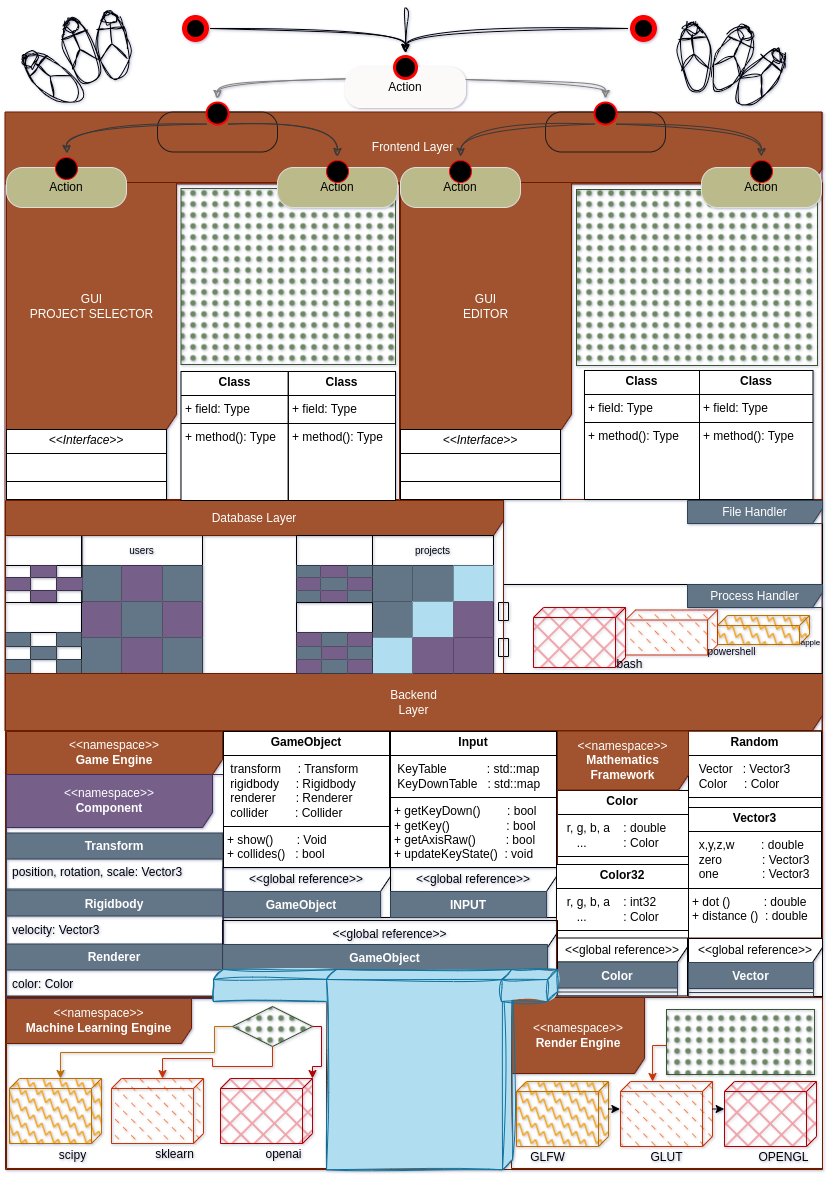
\includegraphics[width=\textwidth]{implementation_arch.png}
      \caption{Arch}
      \end{center}
    \end{figure}

    







    % The software frontend is wrote in PyQt,a python wrapper for the industry standard qt.




\chapter*{pyroGamer - The PyQt Editor}

\section*{Introduction}
The frontend component is called "the PyroGamer project" and is organized into several directories and files. It includes functionalities for the Editor, Hub, and Splash interfaces. These components are managed through various Python scripts and stylesheets. The overall structure can be understood through the following.


\textbf{Directory Structure}

% The directory structure of the frontend is hierarchical. Let \( D \) represent the directory structure where:
\[
  \text{Directory } D := \{d_1, d_2, \ldots, d_n\}
\]
\[
  \text{typeOf} (\( d_i \)) \in \{\text{File}, \text{Directory}\}
\]
% can either be a file or a sub-directory containing further files or sub-directories.

\textbf{Components}

Most of the sub-modules start as this:
\[
F_m = S_m = \{\text{\_\_init\_\_.py}, \text{\_\_main\_\_.py}\}
\]

And then each of them comes with their own required technologies.


% \textbf{\emph{PROJECT LOADER}}

\[
  \text{let hub } H
\xrightarrow{\text{depend}}
\text{cli interface} 
\land 
\text{FileManager} 
\land 
(
\text{gui engine}
\land
\text{icons}
)
% \text{Tabs & Tables}
\]

% \textbf{\emph{Game Editor}}

\[
  \text{let editor } E 
\xrightarrow{\text{depend}}
\text{Hierarchy} 
\land 
\text{SceneView} 
\land 
\text{Inspector}
\land 
(
\text{Assets}
\land 
\text{Terminal}
)
\]

% \subsection*{Editor}
% The Editor component is represented by the set \( E \):
% \[
% E = \{e_1, e_2, \ldots, e_m\}
% \]
% where each \( e_i \) is a sub-directory or file under the Editor directory. Specifically:

\subsubsection*{Configs}
The Configs sub-directory contains scripts for configuration management:
\[
C = \{\text{FileManager.py}, \text{\_\_init\_\_.py}, \text{\_\_main\_\_.py}\}
\]

\begin{lstlisting}[language=Python, caption=FileManager.py]
import os

class FileManager:
    def __init__(self, path):
        self.path = path

    def list_files(self):
        return os.listdir(self.path)
\end{lstlisting}

\subsubsection*{Elements}
The Elements sub-directory is defined as:
\[
L = \{\text{Pages.py}, \text{Tabs}\}
\]
where Tabs itself is a set:
\[
T = \{\text{Assets.py}, \text{Hierarchy.py}, \text{Inspector.py}, \text{SceneView.py}, \text{Terminal.py}\}
\]

\begin{lstlisting}[language=Python, caption=Assets.py]
class AssetsTab:
    def __init__(self):
        self.assets = []

    def add_asset(self, asset):
        self.assets.append(asset)
\end{lstlisting}

\subsubsection*{FileManager and SceneManager}
Both FileManager and SceneManager sub-directories are represented as:
\[
F_m = S_m = \{\text{\_\_init\_\_.py}, \text{\_\_main\_\_.py}\}
\]

\begin{lstlisting}[language=Python, caption=__main__.py]
if __name__ == '__main__':
    print("Initializing Manager")
\end{lstlisting}

\subsubsection*{Styles}
The Styles sub-directory contains CSS files for styling:
\[
S_t = \{\text{createProjWindow.css}, \text{noProjectWindow.css}, \text{projectWindow.css}\}
\]

\subsection*{Hub}
The Hub component is represented by the set \( H \):
\[
H = \{ \text{Configs}, \text{Elements}, \text{icons}, \text{\_\_main\_\_.py} \}
\]

\subsubsection*{Configs}
The Configs sub-directory in Hub contains:
\[
C_h = \{ \text{FileManager.py}, \text{\_\_main\_\_.py} \}
\]

\subsubsection*{Elements}
The Elements sub-directory in Hub is:
\[
L_h = \{ \text{Tables.py}, \text{Tabs.py} \}
\]

\subsection*{Splash}
The Splash component contains:
\[
S_p = \{ \text{images}, \text{\_\_main\_\_.py} \}
\]

\section*{Inter-component Relationships}
The interactions between different components can be represented using functions and mappings. Let \( f: E \to H \) represent the function mapping elements from the Editor to the Hub. Similarly, \( g: H \to S_p \) represents the mapping from Hub to Splash.

\subsection*{File Management}
File management across different components is handled by the scripts in Configs and FileManager directories. Let \( \mathcal{F} \) be the set of file management scripts:
\[
\mathcal{F} = C \cup F_m \cup C_h
\]

\subsection*{Styling}
Styling is governed by CSS files in the Styles directory:
\[
\mathcal{S} = S_t
\]

The overall relationship between these parts can be expressed as:
\[
\text{Frontend} = \mathcal{F} \cup \mathcal{S} \cup (L \cup L_h) \cup S_p
\]

\section*{Conclusion}
The frontend component of PyroGamer is a well-structured combination of directories and files. Each part has a specific role, and their interactions can be mathematically represented to understand the flow and dependencies within the system.

